\section{Heterogeneous Agents and Distributions}

This section studies economies in which households are hit by \emph{idiosyncratic} (individual-specific) income shocks that they cannot fully insure. Because different households experience different shock histories, they end up with different wealth levels, so the economy has a whole \emph{distribution} of agents rather than a single representative agent. We need two tools to describe it:
\begin{itemize}
  \item the \textbf{Hamilton--Jacobi--Bellman (HJB) equation}, which describes the optimal choices of one household, and
  \item the \textbf{Kolmogorov forward (KF) equation}, also called the Fokker--Planck equation, which describes how the cross-sectional distribution of households evolves given those choices.
\end{itemize}
Equilibrium then requires that the prices households take as given (the interest rate, the wage) clear markets once we aggregate over the distribution.

%--------------------------------------------------------------------
\subsection{Huggett model: motivation and setup \pg{39}}

\paragraph{Motivation.}
\begin{itemize}
  \item \textbf{Markets are incomplete.} In the data, only about one third of \emph{permanent} income shocks are insured through markets (or other arrangements); the rest passes through to consumption. A representative-agent model with complete markets cannot capture this.
  \item \textbf{Self-insurance.} In the Huggett model households cannot buy insurance against income shocks. Instead they \emph{self-insure}: they accumulate a \textbf{buffer stock of savings} in good times and run it down in bad times, which smooths consumption against idiosyncratic shocks.
  \item \textbf{Two sources of market incompleteness:}
    \begin{enumerate}
      \item the only asset available for saving or borrowing is a single \emph{risk-free bond} (no state-contingent claims, so no insurance contracts);
      \item there is a \emph{borrowing constraint}: households cannot borrow beyond a limit.
    \end{enumerate}
  \item \textbf{Two kinds of heterogeneity:}
    \begin{itemize}
      \item \emph{ex-ante}: agents differ in fixed characteristics from the start (e.g.\ different preferences or abilities);
      \item \emph{ex-post}: agents are identical ex-ante but become different because they receive different realisations of random shocks.
    \end{itemize}
    Huggett and Aiyagari models use \textbf{ex-post} heterogeneity: everybody faces the same income process, but luck differs.
\end{itemize}

\paragraph{Setup (continuous time).}
\begin{itemize}
  \item Time $t\ge0$ is continuous. There is a continuum of households of total mass $1$.
  \item $a_t$: a household's wealth (bond holdings) at time $t$. $a_t<0$ means the household is a borrower.
  \item $y_t$: the household's labour income (an endowment, no labour choice). It takes two values, $y_t\in\{y_1,y_2\}$ with $y_1<y_2$: $y_1$ is the ``bad'' state (e.g.\ unemployment) and $y_2$ the ``good'' state.
  \item Income follows a two-state \textbf{Poisson process}: a household in state $j$ jumps to the other state at rate $\lambda_j>0$, i.e.\ over a short interval of length $\Delta$ it switches with probability $\lambda_j\Delta$ and stays with probability $1-\lambda_j\Delta$ (up to terms of order $\Delta^2$). We write $-j$ for ``the other state'' (if $j=1$ then $-j=2$ and vice versa). Later the income process is generalised, e.g.\ to a diffusion.
  \item $c_t$: consumption, chosen by the household. $u(\cdot)$: instantaneous utility, strictly increasing and strictly concave ($u'>0$, $u''<0$). $\rho>0$: discount rate.
  \item $r$: the interest rate on the bond. The household takes $r$ as given; in equilibrium it is determined by market clearing.
  \item $\underline a$: the borrowing limit (exogenous).
\end{itemize}

The household solves
\begin{equation}\label{eq:hug-problem}
  \max_{\{c_t\}_{t\ge0}} \; E_0\!\int_0^\infty e^{-\rho t}u(c_t)\,dt
  \quad\text{s.t.}\quad
  \dot a_t = y_t + r a_t - c_t,\qquad a_t\ge \underline a ,
\end{equation}
where $\dot a_t\equiv da_t/dt$. The budget constraint says wealth grows by income plus interest minus consumption.

\paragraph{The borrowing limit and the natural borrowing limit.}
We require $\underline a\ge -y_1/r$ (for $r>0$). To see where $-y_1/r$ comes from, ask: what is the largest debt a household could \emph{surely} repay? In the worst case its income stays at $y_1$ forever. The present value of that income stream is
\begin{align*}
  \int_0^\infty e^{-rt}y_1\,dt
  &= y_1\Big[-\tfrac{1}{r}e^{-rt}\Big]_0^\infty &&\text{(integrate the exponential)}\\
  &= \frac{y_1}{r}. &&\text{(}e^{-rt}\to0\text{ as }t\to\infty\text{)}
\end{align*}
Even consuming (almost) nothing, the household can repay at most $y_1/r$, so lenders would never lend more: debt must satisfy $-a_t\le y_1/r$, i.e.\ $a_t\ge -y_1/r$. This is the \textbf{natural borrowing limit}. Any \emph{ad hoc} limit $\underline a$ must be at least as tight: $\underline a\ge -y_1/r$.
\begin{itemize}
  \item Special case $\underline a=0$: households can only save, never borrow.
\end{itemize}

\paragraph{Equilibrium concept.} In \textbf{general equilibrium}, bonds are in \textbf{zero net supply}: they are IOUs between households, so total borrowing must equal total lending, i.e.\ aggregate wealth is zero. The interest rate $r$ adjusts to make this hold.

%--------------------------------------------------------------------
\subsection{The HJB equation with Poisson income switching \pg{40}}

Let $v_j(a)$ be the value (maximised expected lifetime utility) of a household with wealth $a$ and current income $y_j$. Since the problem is stationary (nothing depends on calendar time given $r$), $v_j$ depends only on $(a,j)$.

\paragraph{Derivation (heuristic, via a short time step).}
Consider a short interval of length $\Delta$. The household consumes $c$, so wealth moves from $a$ to $a+\Delta(y_j+ra-c)$. With probability $1-\lambda_j\Delta$ income stays at $y_j$; with probability $\lambda_j\Delta$ it switches to $y_{-j}$. The discrete-time Bellman equation is
\begin{equation*}
  v_j(a)=\max_c\Big\{\Delta\,u(c) + e^{-\rho\Delta}\Big[(1-\lambda_j\Delta)\,v_j\big(a+\Delta s\big) + \lambda_j\Delta\, v_{-j}\big(a+\Delta s\big)\Big]\Big\},
  \qquad s\equiv y_j+ra-c.
\end{equation*}
Use the first-order approximations $e^{-\rho\Delta}\approx 1-\rho\Delta$ and $v_j(a+\Delta s)\approx v_j(a)+v_j'(a)\Delta s$ (Taylor expansion), and drop all terms of order $\Delta^2$:
\begin{align*}
  v_j(a) &= \max_c\Big\{\Delta u(c) + (1-\rho\Delta)\big[v_j(a)+v_j'(a)\Delta s - \lambda_j\Delta v_j(a) + \lambda_j\Delta v_{-j}(a)\big]\Big\}\\
  &= \max_c\Big\{\Delta u(c) + v_j(a) - \rho\Delta v_j(a) + v_j'(a)\Delta s + \lambda_j\Delta\big(v_{-j}(a)-v_j(a)\big)\Big\}.
\end{align*}
Subtract $v_j(a)$ from both sides, move $\rho\Delta v_j(a)$ to the left and divide by $\Delta$:
\begin{equation}\label{eq:hug-hjb}
  \rho v_j(a) = \max_c\Big\{u(c) + v_j'(a)\,(y_j+ra-c) + \lambda_j\big(v_{-j}(a)-v_j(a)\big)\Big\},\qquad j=1,2.
\end{equation}

\textbf{Reading the HJB.} The left side is the ``return'' on the value $v_j$ at rate $\rho$. The right side is the flow payoff: utility $u(c)$, plus the value of the change in wealth ($v_j'(a)\times\dot a$), plus the expected capital gain or loss from a switch in income: with intensity $\lambda_j$ the value jumps from $v_j(a)$ to $v_{-j}(a)$.

\paragraph{Optimal consumption.} Maximising the right side of \eqref{eq:hug-hjb} over $c$ gives the first-order condition
\begin{equation}\label{eq:hug-foc}
  u'\big(c_j(a)\big) = v_j'(a)\quad\Longrightarrow\quad c_j(a)=(u')^{-1}\big(v_j'(a)\big).
\end{equation}
The marginal utility of consuming one more unit equals the marginal value of keeping it as wealth. The implied \textbf{saving policy} in state $j$ is
\begin{equation}\label{eq:hug-saving}
  s_j(a)\equiv y_j + ra - c_j(a)\quad(=\dot a\text{ for a household in state }j\text{ with wealth }a).
\end{equation}

%--------------------------------------------------------------------
\subsection{Kolmogorov forward equation with Poisson shocks \pg{40}}

Given the policies $s_j(a)$, we now track how the population distributes itself over wealth and income.

\paragraph{Setup.}
\begin{itemize}
  \item $\tilde a_t,\tilde y_t$: wealth and income of a randomly drawn household at time $t$ (tildes denote random variables).
  \item Joint CDF in income state $j$:\quad $G_j(a,t)\equiv\Pr\big(\tilde a_t\le a,\ \tilde y_t=y_j\big)$.
  \item Density: $g_j(a,t)\equiv\partial_a G_j(a,t)$, so $g_j(a,t)\,da$ is the mass of households with income $y_j$ and wealth in $[a,a+da]$. Here $\partial_a$ and $\partial_t$ denote partial derivatives in the wealth and time dimensions.
  \item Note $G_1+G_2$ is the marginal CDF of wealth, and $\int (g_1+g_2)\,da=1$.
\end{itemize}

\paragraph{Step 1: the law of motion over a short interval.}
Over an interval of length $\Delta$, a household in state $j$ moves deterministically along its saving policy, $\tilde a_{t+\Delta}=\tilde a_t+\Delta\,s_j(\tilde a_t)$, and its income switches to $-j$ with probability $\lambda_j\Delta$.

Which households are in state $j$ with wealth $\le a$ at $t+\Delta$? Two groups:
\begin{itemize}
  \item households that were in $j$ and did \emph{not} switch (probability $1-\lambda_j\Delta$) and whose wealth satisfies $\tilde a_t+\Delta s_j(\tilde a_t)\le a$, i.e.\ (to first order) $\tilde a_t\le a-\Delta s_j(a)$;
  \item households that were in $-j$ and \emph{did} switch into $j$ (probability $\lambda_{-j}\Delta$), with $\tilde a_t\le a-\Delta s_{-j}(a)$.
\end{itemize}
Hence
\begin{equation}\label{eq:kf-discrete}
  G_j(a,t+\Delta) = (1-\lambda_j\Delta)\,G_j\big(a-\Delta s_j(a),t\big) + \lambda_{-j}\Delta\,G_{-j}\big(a-\Delta s_{-j}(a),t\big).
\end{equation}

\paragraph{Step 2: take the limit $\Delta\to0$.}
Taylor-expand in the wealth argument: $G_j(a-\Delta s_j(a),t)\approx G_j(a,t)-\Delta s_j(a)\,\partial_aG_j(a,t)$. Substitute into \eqref{eq:kf-discrete}:
\begin{align*}
  G_j(a,t+\Delta) &= (1-\lambda_j\Delta)\big[G_j(a,t)-\Delta s_j(a)\partial_aG_j(a,t)\big] + \lambda_{-j}\Delta\,G_{-j}(a,t) + O(\Delta^2)\\
  &= G_j(a,t) - \Delta s_j(a)\partial_aG_j(a,t) - \lambda_j\Delta G_j(a,t) + \lambda_{-j}\Delta G_{-j}(a,t) + O(\Delta^2).
\end{align*}
Subtract $G_j(a,t)$ from both sides and divide by $\Delta$:
\begin{equation*}
  \frac{G_j(a,t+\Delta)-G_j(a,t)}{\Delta} = - s_j(a)\partial_aG_j(a,t) - \lambda_j G_j(a,t) + \lambda_{-j} G_{-j}(a,t) + O(\Delta).
\end{equation*}
Let $\Delta\to0$; the left side becomes $\partial_tG_j(a,t)$:
\begin{equation}\label{eq:kf-cdf}
  \partial_t G_j(a,t) = -s_j(a)\,\partial_a G_j(a,t) - \lambda_j G_j(a,t) + \lambda_{-j}G_{-j}(a,t).
\end{equation}

\paragraph{Step 3: from the CDF to the density.}
Differentiate \eqref{eq:kf-cdf} with respect to $a$. On the left, $\partial_a\partial_tG_j=\partial_t\partial_aG_j=\partial_t g_j$. On the right, $\partial_a\big[s_j(a)\partial_aG_j\big]=\partial_a\big[s_j(a)g_j\big]$ and $\partial_aG_{\pm j}=g_{\pm j}$. Therefore
\begin{keybox}[title=Kolmogorov forward equation (two-state Poisson income)]
\begin{equation}\label{eq:kf-density}
  \partial_t g_j(a,t) = -\partial_a\big[s_j(a)\,g_j(a,t)\big] \;-\; \underbrace{\lambda_j g_j(a,t)}_{\text{outflow from }j} \;+\; \underbrace{\lambda_{-j}g_{-j}(a,t)}_{\text{inflow from }-j},\qquad j=1,2.
\end{equation}
\end{keybox}
\textbf{Interpretation.} The density at $(a,j)$ changes for two reasons. (i) \emph{Drift in the wealth dimension}: $-\partial_a[s_jg_j]$ is minus the derivative of the flow of households moving through wealth level $a$ (the ``flux'' $s_jg_j$); if more households flow out of a small wealth interval than flow in, the density there falls. (ii) \emph{Jumps in the income dimension}: households in $j$ leave at rate $\lambda_j$, and households in $-j$ arrive at rate $\lambda_{-j}$.

\paragraph{Implied stationary income distribution.}
Let $\pi_j(t)\equiv\int g_j(a,t)\,da$ be the share of households in income state $j$. Integrate \eqref{eq:kf-density} over all $a$. The drift term integrates to the net flux through the boundaries of the wealth space, $-[s_jg_j]_{\underline a}^{\infty}$, which is zero because no household leaves the state space (at $\underline a$ wealth cannot fall, and $g_j\to0$ as $a\to\infty$). So
\begin{equation*}
  \dot\pi_j(t) = -\lambda_j\pi_j(t)+\lambda_{-j}\pi_{-j}(t).
\end{equation*}
In a stationary state $\dot\pi_j=0$, so $\lambda_1\pi_1=\lambda_2\pi_2$; with $\pi_1+\pi_2=1$ this gives
\begin{equation}\label{eq:pi-stat}
  \pi_1=\frac{\lambda_2}{\lambda_1+\lambda_2},\qquad \pi_2=\frac{\lambda_1}{\lambda_1+\lambda_2}.
\end{equation}
The flow out of the bad state equals the flow into it; the bad state is more common when it is hard to leave ($\lambda_1$ small) and easy to enter ($\lambda_2$ large).

%--------------------------------------------------------------------
\subsection{Huggett stationary equilibrium \pg{40}}

A \textbf{stationary} equilibrium is one in which the distribution no longer changes over time: $\partial_t g_j(a,t)=0$. We then drop the $t$ argument and write $g_j(a)$. Setting the left side of \eqref{eq:kf-density} to zero removes the time dimension, and the partial derivative in $a$ becomes an ordinary derivative.

\begin{keybox}[title=Huggett stationary equilibrium]
An interest rate $r$, value functions $v_j$, policies $c_j,s_j$ and densities $g_j$ ($j=1,2$) such that:
\begin{align}
  \text{(HJB)}\quad & \rho v_j(a) = \max_c\Big\{u(c) + v_j'(a)\,(y_j+ra-c) + \lambda_j\big(v_{-j}(a)-v_j(a)\big)\Big\},\label{eq:hug-eq-hjb}\\
  \text{(KF)}\quad & 0 = -\frac{d}{da}\big[s_j(a)\,g_j(a)\big] - \lambda_j g_j(a) + \lambda_{-j}g_{-j}(a),\label{eq:hug-eq-kf}\\
  \text{(density)}\quad & \int_{\underline a}^\infty \big(g_1(a)+g_2(a)\big)\,da = 1,\qquad g_1,g_2\ge 0,\label{eq:hug-eq-dens}\\
  \text{(bond market)}\quad & S(r) \equiv \int_{\underline a}^\infty a\,g_1(a)\,da + \int_{\underline a}^\infty a\,g_2(a)\,da = 0,\label{eq:hug-eq-mkt}
\end{align}
with $s_j(a)=y_j+ra-c_j(a)$ and $u'(c_j(a))=v_j'(a)$ from \eqref{eq:hug-foc}.
\end{keybox}
\begin{itemize}
  \item The HJB gives individual behaviour for a given $r$; the KF equation aggregates that behaviour into a distribution; the density condition normalises total mass to one.
  \item $S(r)$ is aggregate wealth (aggregate saving) at interest rate $r$. Because bonds are in zero net supply, $S(r)=0$: total lending (positive $a$) equals total borrowing (negative $a$).
  \item The system is recursive in $r$: given $r$ we can solve \eqref{eq:hug-eq-hjb}, then \eqref{eq:hug-eq-kf}--\eqref{eq:hug-eq-dens}, then evaluate $S(r)$. Equilibrium is the $r$ that sets $S(r)=0$.
\end{itemize}

%--------------------------------------------------------------------
\subsection{The borrowing constraint as a boundary condition \pg{40--41}}

The constraint $a\ge\underline a$ is imposed at the \textbf{lower boundary} of the wealth space, as a condition on the value function at $a=\underline a$. This is how it enters the numerical (finite-difference) code.

\paragraph{Step 1: saving at the constraint cannot be negative.}
A household sitting exactly at $a=\underline a$ cannot let its wealth fall further. So its saving there must be non-negative:
\begin{equation}\label{eq:bc-saving}
  s_j(\underline a) = y_j + r\underline a - c_j(\underline a) \;\ge\; 0 .
\end{equation}
If instead $s_j(\underline a)<0$, wealth would fall below $\underline a$ an instant later, which is impossible in the model.

\paragraph{Step 2: translate into a condition on $v_j'(\underline a)$.}
Rearranging \eqref{eq:bc-saving}: $c_j(\underline a)\le y_j+r\underline a$. Since $u$ is concave, $u'$ is decreasing, so a smaller argument gives a larger marginal utility:
\begin{align*}
  c_j(\underline a)\le y_j+r\underline a
  &\;\Longrightarrow\; u'\big(c_j(\underline a)\big)\ \ge\ u'\big(y_j+r\underline a\big) &&\text{(}u'\text{ decreasing)}\\
  &\;\Longrightarrow\; v_j'(\underline a)\ \ge\ u'\big(y_j+r\underline a\big). &&\text{(FOC \eqref{eq:hug-foc} at }a=\underline a\text{)}
\end{align*}
\begin{keybox}[title=State-constraint boundary condition]
\begin{equation}\label{eq:state-constraint}
  v_j'(\underline a)\;\ge\;u'\big(y_j+r\underline a\big),\qquad j=1,2.
\end{equation}
\end{keybox}
\textbf{Interpretation.} At the borrowing limit the marginal value of wealth is at least the marginal utility of consuming all current income. In practice, in the finite-difference scheme the derivative at the boundary is set to $v_j'(\underline a)=u'(y_j+r\underline a)$ whenever the unconstrained choice would imply dissaving, which forces $c_j(\underline a)= y_j+r\underline a$ and $s_j(\underline a)=0$. Typically the constraint binds for low-income households: they would like to borrow more but cannot, and a mass of them sits at $\underline a$.

%--------------------------------------------------------------------
\subsection{Variations: Huggett, Bewley and Aiyagari \pg{41--42}}

All three models share the same household block (HJB + KF); they differ in \emph{what the asset is} and therefore in the market-clearing condition. Write $A(r)$ for aggregate household asset demand at interest rate $r$ (in Huggett, $A(r)=S(r)$ from \eqref{eq:hug-eq-mkt}).

\subsubsection*{(a) Huggett: assets in zero net supply}
Equilibrium condition: $A(r)=0$. \textbf{Computation} by iterating on the interest rate:
\begin{enumerate}
  \item Guess $r$.
  \item Solve the HJB \eqref{eq:hug-eq-hjb} for $v_j$, hence $c_j(a)$ and $s_j(a)$.
  \item Solve the KF equation \eqref{eq:hug-eq-kf} with \eqref{eq:hug-eq-dens} for $g_j$.
  \item Compute $S(r)$ from \eqref{eq:hug-eq-mkt}.
  \item If $S(r)>0$ (excess saving), lower $r$; if $S(r)<0$ (excess borrowing), raise $r$. Return to step 2 until $S(r)\approx0$ (e.g.\ by bisection).
\end{enumerate}
This works because $S(r)$ is increasing in $r$: a higher return makes households save more and borrow less.

\begin{center}
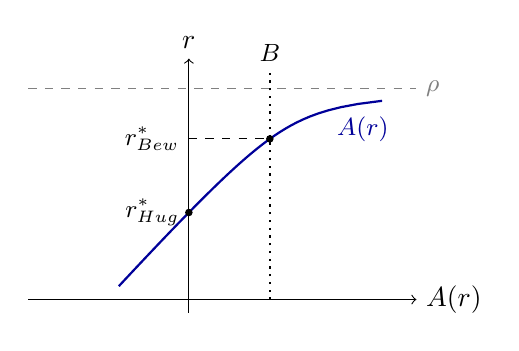
\begin{tikzpicture}[scale=0.85]
  \draw[->] (-2.4,0)--(3.4,0) node[right]{$A(r)$};
  \draw[->] (0,-0.2)--(0,3.6) node[above]{$r$};
  \draw[dashed,gray] (-2.4,3.15)--(3.4,3.15) node[right]{\small $\rho$};
  \draw[thick,blue!60!black,domain=0.2:2.97,samples=60,variable=\t]
     plot ({0.15*(\t-1.3)/(3.15-\t)+0.9*(\t-1.3)},{\t});
  \node[blue!60!black] at (2.6,2.55) {\small $A(r)$};
  \fill (0,1.3) circle (1.6pt) node[left]{\small $r^*_{\text{Hug}}$};
  \draw[dotted,thick] (1.21,0)--(1.21,3.4) node[above]{\small $B$};
  \fill (1.21,2.4) circle (1.6pt);
  \draw[dashed] (0,2.4)--(1.21,2.4);
  \node[left] at (0,2.4) {\small $r^*_{\text{Bew}}$};
\end{tikzpicture}
\end{center}
\textbf{How to read the figure.} The horizontal axis is aggregate asset demand, the vertical axis the interest rate. The curve $A(r)$ slopes up because a higher $r$ raises saving; it diverges to $+\infty$ as $r\uparrow\rho$ because when the return on saving approaches the rate of time preference, households keep accumulating buffer-stock wealth without bound. Huggett's equilibrium is where $A(r)$ crosses the vertical axis ($A=0$); with positive bond supply $B$ (Bewley, below) the equilibrium is where $A(r)$ meets the vertical line at $B$, so $r^*_{\text{Bew}}>r^*_{\text{Hug}}$.

\subsubsection*{(b) Bewley: assets in positive supply}
\textbf{Setup.}
\begin{itemize}
  \item The government issues an exogenous amount $B>0$ of bonds, which households hold. A larger $B$ affects the equilibrium $r$ (see figure).
  \item It finances interest payments $rB$ and government spending $G$ by collecting taxes according to a tax function $\tau(a,y)$ (tax paid by a household with wealth $a$ and income $y$).
  \item $g(a,y_j;r)$: stationary density over $(a,y_j)$ when the interest rate is $r$ (same as $g_j(a)$ above, with the dependence on $r$ made explicit).
\end{itemize}
\textbf{Conditions.}
\begin{align*}
  \text{Total tax revenue:}\quad & T(r)=\sum_j\int_a \tau(a,y_j)\,g(a,y_j;r)\,da,\\
  \text{Government budget constraint:}\quad & G(r)+rB=T(r),\\
  \text{Asset market clearing:}\quad & A(r)=B.
\end{align*}
Given $B$ and the tax function, spending $G(r)$ is whatever the budget constraint allows. Households must now be willing to hold the positive stock $B$, which requires a higher interest rate than in Huggett.

\subsubsection*{(c) Aiyagari: adding production}
\textbf{Setup.}
\begin{itemize}
  \item A representative firm with constant-returns-to-scale (CRS) technology, and no aggregate shocks:
  $Y=K^\alpha L^{1-\alpha}$, $0<\alpha<1$; $K$: capital, $L$: effective labour.
  \item Capital depreciates at rate $\delta$. The firm rents capital at rental rate $r+\delta$ (households earn $r$ net of depreciation) and hires labour at wage $w$. Markets are competitive.
  \item Households own the capital: their wealth $a$ is now claims on $K$, so the asset is in \emph{positive} supply determined by the firm's demand for capital.
\end{itemize}

\paragraph{Firm optimisation.} The firm solves $\max_{K,L}\ K^\alpha L^{1-\alpha}-(r+\delta)K-wL$. The first-order conditions set factor prices equal to marginal products:
\begin{align}
  \partial_K:\quad & r+\delta=\alpha K^{\alpha-1}L^{1-\alpha}=\alpha\Big(\frac{K}{L}\Big)^{\alpha-1},\label{eq:aiy-r}\\
  \partial_L:\quad & w=(1-\alpha)K^{\alpha}L^{-\alpha}=(1-\alpha)\Big(\frac{K}{L}\Big)^{\alpha}.\label{eq:aiy-w}
\end{align}
Solve \eqref{eq:aiy-r} for the capital--labour ratio:
\begin{align*}
  \Big(\frac{K}{L}\Big)^{\alpha-1}&=\frac{r+\delta}{\alpha}
  &&\text{(divide by }\alpha\text{)}\\
  \frac{K}{L}&=\Big(\frac{r+\delta}{\alpha}\Big)^{\frac{1}{\alpha-1}}=\Big(\frac{\alpha}{r+\delta}\Big)^{\frac{1}{1-\alpha}}.
  &&\text{(raise to the power }1/(\alpha-1)\text{)}
\end{align*}
Substitute into \eqref{eq:aiy-w}:
\begin{equation}\label{eq:aiy-wr}
  w(r)=(1-\alpha)\Big(\frac{\alpha}{r+\delta}\Big)^{\frac{\alpha}{1-\alpha}}.
\end{equation}
So the wage is pinned down by $r$ alone (CRS means only the ratio $K/L$ matters), and $w'(r)<0$: a higher cost of capital means less capital per worker and a lower wage. Hence the whole model can again be solved by iterating on a single price $r$.

\paragraph{Household problem (discrete-time version).} With labour productivity $y_j$ (the household supplies $y_j$ efficiency units of labour inelastically), the budget constraint is
\begin{equation*}
  c+a'=w\,y_j+(1+r)a,\qquad a'\ge\underline a,
\end{equation*}
where $a'$ is next period's wealth. The household problem is exactly Huggett's, with income $w y_j$ instead of $y_j$.

\paragraph{Two market-clearing conditions.}
\begin{itemize}
  \item \textbf{Labour market} (labour supply is exogenous):
  \begin{equation}\label{eq:aiy-L}
    L=\sum_j\int_a y_j\,g(a,y_j;r)\,da=\sum_j y_j\int_a g(a,y_j;r)\,da=\sum_j y_j\pi_j,
  \end{equation}
  where $\pi_j\equiv\int_a g(a,y_j;r)\,da$ is the stationary share of households with productivity $y_j$ (for the two-state Poisson process, \eqref{eq:pi-stat}). Since $\pi_j$ depends only on the exogenous income process, $L$ does not depend on $r$.
  \item \textbf{Capital market}: household asset supply equals firm capital demand. Multiplying the capital--labour ratio by $L$,
  \begin{equation}\label{eq:aiy-K}
    A(r)=K(r)\equiv L\Big(\frac{\alpha}{r+\delta}\Big)^{\frac{1}{1-\alpha}}.
  \end{equation}
\end{itemize}

\begin{center}
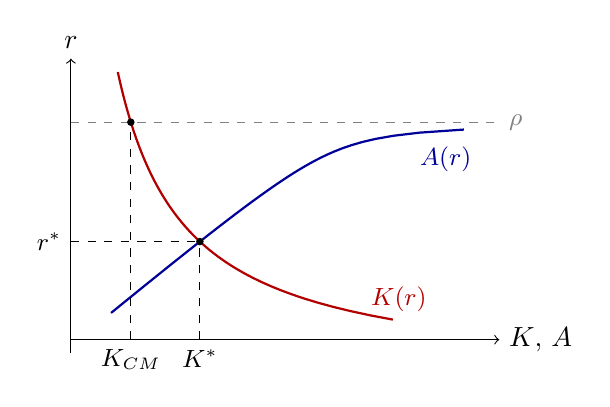
\begin{tikzpicture}[scale=0.85]
  \draw[->] (0,0)--(6.4,0) node[right]{$K$, $A$};
  \draw[->] (0,-0.2)--(0,4.2) node[above]{$r$};
  \draw[dashed,gray] (0,3.25)--(6.4,3.25) node[right]{\small $\rho$};
  \draw[thick,blue!60!black,domain=0.4:3.14,samples=60,variable=\t]
     plot ({0.6+1.2*(\t-0.4)+0.08*(\t-0.4)/(3.25-\t)},{\t});
  \node[blue!60!black] at (5.6,2.7) {\small $A(r)$};
  \draw[thick,red!70!black,domain=0.3:4.0,samples=60,variable=\t]
     plot ({4.6/(\t+0.6)-0.3},{\t});
  \node[red!70!black] at (4.9,0.6) {\small $K(r)$};
  \fill (1.927,1.466) circle (1.6pt);
  \draw[dashed] (0,1.466)--(1.927,1.466); \node[left] at (0,1.466) {\small $r^*$};
  \draw[dashed] (1.927,0)--(1.927,1.466); \node[below] at (1.927,0) {\small $K^*$};
  \fill (0.895,3.25) circle (1.6pt);
  \draw[dashed] (0.895,0)--(0.895,3.25); \node[below] at (0.895,0) {\small $K_{\text{CM}}$};
\end{tikzpicture}
\end{center}
\textbf{How to read the figure.} The red curve $K(r)$ is firms' capital demand from \eqref{eq:aiy-K}; it slopes down because a higher rental cost lowers the desired capital stock. The blue curve $A(r)$ is households' aggregate asset supply from the HJB+KF block; it slopes up and explodes as $r\uparrow\rho$. Their intersection gives $(r^*,K^*)$. Under complete markets (representative agent) the steady-state interest rate would be $r=\rho$, giving the smaller capital stock $K_{\text{CM}}$ where $K(r)$ reaches $\rho$; precautionary saving pushes $r^*<\rho$ and $K^*>K_{\text{CM}}$.

\paragraph{Continuous-time Aiyagari with diffusion income.}
\textbf{Setup.} Replace the two-state income process by a continuous productivity $z\in[z_{\min},z_{\max}]$ following a diffusion
\begin{equation*}
  dz_t=\mu(z_t)\,dt+\sigma(z_t)\,dW_t,
\end{equation*}
where $\mu(z)$ is the drift, $\sigma(z)$ the volatility, and $W_t$ a standard Brownian motion. Labour income is $wz$, so wealth evolves as $\dot a=wz+ra-c$, and the saving policy is $s(a,z)=wz+ra-c(a,z)$. The value function is $V(a,z)$ and the stationary density $g(a,z)$.

\emph{Ito's lemma} (used for the HJB): if $dz=\mu\,dt+\sigma\,dW$ and $a$ moves deterministically, then $E[dV]=\big(\partial_aV\,\dot a+\mu\,\partial_zV+\tfrac12\sigma^2\partial_{zz}V\big)dt$. Replacing the Poisson jump term in \eqref{eq:hug-hjb} by this expected drift of $V$ gives the HJB below. The KF equation is the ``adjoint'' of the HJB operator: each derivative acting on $V$ becomes a derivative of (coefficient $\times\, g$) with the sign flipped for first derivatives.

\begin{keybox}[title={Aiyagari stationary system (continuous time, diffusion income)}]
\begin{align}
  \text{(HJB)}\quad & \rho V(a,z) = \max_c\Big\{u(c) + \partial_aV(a,z)\,(wz+ra-c) + \mu(z)\,\partial_zV(a,z) \notag\\
  &\hspace{8.5em} + \tfrac12\sigma^2(z)\,\partial_{zz}V(a,z)\Big\},\label{eq:aiy-hjb}\\
  \text{(KF)}\quad & 0 = -\partial_a\big[s(a,z)g(a,z)\big] - \partial_z\big[\mu(z)g(a,z)\big] + \tfrac12\partial_{zz}\big[\sigma^2(z)g(a,z)\big],\label{eq:aiy-kf}\\
  \text{(density)}\quad & 1 = \int_{z_{\min}}^{z_{\max}}\!\!\int_{\underline a}^\infty g(a,z)\,da\,dz,\label{eq:aiy-dens}\\
  \text{(capital supply)}\quad & K = \int_{z_{\min}}^{z_{\max}}\!\!\int_{\underline a}^\infty a\,g(a,z)\,da\,dz,\label{eq:aiy-Ksupply}\\
  \text{(market clearing)}\quad & K = L\Big(\frac{\alpha}{r+\delta}\Big)^{\frac{1}{1-\alpha}},\qquad L=\int_{z_{\min}}^{z_{\max}}\!\!\int_{\underline a}^\infty z\,g(a,z)\,da\,dz,\label{eq:aiy-clear}
\end{align}
with $w=w(r)$ from \eqref{eq:aiy-wr}, the FOC $u'(c(a,z))=\partial_aV(a,z)$, and the state-constraint condition $\partial_aV(\underline a,z)\ge u'(wz+r\underline a)$.
\end{keybox}
\textbf{Interpretation.} \eqref{eq:aiy-kf} is \eqref{eq:kf-density} with the Poisson jump terms replaced by drift and diffusion in $z$, and $\partial_t g=0$ imposed. The first integral normalises the distribution; the second aggregates household wealth into the capital stock; the last line requires that this capital equals what firms demand at $r$.

\begin{tipbox}
The algorithm is always the same: guess the price $r$ (and hence $w(r)$) $\to$ solve the HJB $\to$ solve the KF equation $\to$ aggregate $\to$ check market clearing ($A=0$, $A=B$ or $A=K(r)$) $\to$ update $r$. Precautionary saving pushes $r$ below $\rho$: at $r=\rho$ households facing uninsurable risk and a borrowing limit would accumulate wealth without bound, so asset supply can equal any finite demand only at some $r<\rho$. In Aiyagari this means $K$ exceeds its complete-markets level.
\end{tipbox}

%--------------------------------------------------------------------
\subsection{Power laws, Pareto distribution and Zipf's law \pg{96}}

Many economic size variables (wealth, firm size, city size) have very fat right tails. Power laws are the standard way to describe them.

\paragraph{Setup.}
\begin{itemize}
  \item $S$: a positive random variable (``size''), with realisations $s$.
  \item $s_m>0$: the minimum possible value of $s$ (the scale parameter).
  \item $\alpha>0$: the shape (tail) parameter.
  \item $N$: number of observations (e.g.\ number of cities).
\end{itemize}

\paragraph{Pareto distribution.} The density is
\begin{equation}\label{eq:pareto-pdf}
  f(s)=\frac{\alpha s_m^\alpha}{s^{\alpha+1}}=\alpha s_m^\alpha s^{-\alpha-1},\qquad s\ge s_m.
\end{equation}
\emph{CDF.} Integrate the density from the minimum:
\begin{align*}
  F(s)&=\int_{s_m}^{s}\alpha s_m^\alpha x^{-\alpha-1}\,dx\\
  &=\alpha s_m^\alpha\Big[\frac{x^{-\alpha}}{-\alpha}\Big]_{s_m}^{s} &&\text{(antiderivative of }x^{-\alpha-1}\text{)}\\
  &=s_m^\alpha\big(s_m^{-\alpha}-s^{-\alpha}\big)\\
  &=1-\Big(\frac{s_m}{s}\Big)^\alpha.
\end{align*}
\emph{Survival function} (probability of exceeding $s$):
\begin{equation}\label{eq:pareto-surv}
  \bar S(s)\equiv\Pr(S>s)=1-F(s)=\Big(\frac{s_m}{s}\Big)^\alpha .
\end{equation}
Taking logs,
\begin{equation}\label{eq:pareto-logsurv}
  \log\bar S(s)=\alpha\log\Big(\frac{s_m}{s}\Big)=\alpha\log s_m-\alpha\log s .
\end{equation}
\begin{itemize}
  \item The Pareto is a \textbf{long-tailed} distribution: $\bar S(s)$ decays only like a power of $s$, not exponentially.
  \item $\alpha\uparrow\Rightarrow$ the survival function falls faster $\Rightarrow$ thinner tail $\Rightarrow$ lower probability of extreme values. (The mean is finite only if $\alpha>1$, the variance only if $\alpha>2$.)
\end{itemize}

\paragraph{Rank--size relation.}
With $N$ observations, the \textbf{rank} $R(s)$ of an observation of size $s$ is the number of observations larger than $s$ (the largest has rank $\approx1$). For large $N$ this is $N$ times the probability of exceeding $s$:
\begin{equation}\label{eq:rank}
  R(s)=N\,\bar S(s)=N\Big(\frac{s_m}{s}\Big)^\alpha .
\end{equation}
Take logs of \eqref{eq:rank} and use \eqref{eq:pareto-logsurv}:
\begin{align*}
  \log R(s)&=\log N+\log\bar S(s)\\
  &=\underbrace{\log N+\alpha\log s_m}_{\text{constant}}-\alpha\log s .
\end{align*}
\begin{keybox}[title=Log rank vs.\ log size]
Under a Pareto distribution, a plot of $\log(\text{rank})$ against $\log(\text{size})$ is a \textbf{straight line with slope $-\alpha$}. This is how the tail exponent is estimated in practice.
\end{keybox}

\paragraph{Power law (PL).} A more general way to state the same idea: $S$ follows a power law if there exist constants $k,\zeta>0$ such that
\begin{equation}\label{eq:pl}
  \Pr(S>x)=k\,x^{-\zeta}\qquad\text{for all } x\ge x_m,
\end{equation}
where $x_m\equiv k^{1/\zeta}$. The restriction $x\ge x_m$ is needed: a probability cannot exceed one, and $kx^{-\zeta}\le1\iff x\ge k^{1/\zeta}$. In empirical work ``power law'' usually means \eqref{eq:pl} holds in the upper tail (for large $x$).
\begin{itemize}
  \item $\zeta$ smaller $\Rightarrow$ $\Pr(S>x)$ decays more slowly $\Rightarrow$ fatter tail $\Rightarrow$ more inequality (more mass in very large values).
  \item \textbf{Relation to Pareto.} Comparing \eqref{eq:pl} with \eqref{eq:pareto-surv}, $(x_m/x)^\alpha=x_m^\alpha x^{-\alpha}$, so the Pareto distribution is the power law with $\zeta=\alpha$ and $k=x_m^{\zeta}$. Conversely an exact power law on $[x_m,\infty)$ is a Pareto distribution; a variable that only satisfies \eqref{eq:pl} in its tail is ``Pareto in the tail''.
\end{itemize}

\paragraph{Zipf's law.} Zipf's law is the special case $\zeta=1$:
\begin{equation*}
  \Pr(S>x)=\frac{k}{x}\;\propto\;\frac1x :
\end{equation*}
the probability that the variable exceeds a threshold $x$ is inversely proportional to $x$.

\emph{Equivalent rank form.} Let $S_{(r)}$ denote the size of the element with rank $r$ ($r$-th largest). By \eqref{eq:rank}, $r=N\Pr(S>S_{(r)})=N k\,S_{(r)}^{-\zeta}$. Solve for $S_{(r)}$:
\begin{align*}
  S_{(r)}^{\zeta}&=\frac{Nk}{r} &&\text{(multiply by }S_{(r)}^{\zeta}/r\text{)}\\
  S_{(r)}&=\Big(\frac{Nk}{r}\Big)^{1/\zeta}\;\propto\;r^{-1/\zeta}. &&\text{(raise to the power }1/\zeta\text{)}
\end{align*}
Under Zipf ($\zeta=1$) this becomes $S_{(r)}\propto 1/r$: the size (or frequency) of an element is \textbf{inversely proportional to its rank}. The 2nd largest is half the size of the largest, the 3rd largest a third, and so on.

\paragraph{The city size ``puzzle''.} City sizes follow a power law with exponent $\zeta\approx1$, i.e.\ Zipf's law.
\begin{center}
\begin{tikzpicture}[scale=0.8]
  \draw[->] (0,0)--(5,0) node[right]{\small $\ln$ population};
  \draw[->] (0,0)--(0,3.6) node[above]{\small $\ln$ rank};
  \foreach \x/\y in {0.7/2.95,1.1/2.62,1.5/2.40,1.9/2.08,2.3/1.85,2.7/1.52,3.1/1.30,3.5/0.98,3.9/0.72,4.2/0.55}
    \fill[gray] (\x,\y) circle (1.3pt);
  \draw[thick,blue!60!black] (0.5,3.1)--(4.4,0.4) node[right]{\small slope $\approx-1$};
\end{tikzpicture}
\end{center}
\textbf{How to read the figure.} Each dot is a city: horizontal position is log population, vertical position is log rank (the largest city has rank 1, so $\ln\text{rank}=0$ at the far right). By the keybox above, under a power law the dots lie on a straight line whose slope is $-\zeta$. For US cities (Gabaix 1999) the fitted line is
\begin{equation*}
  \ln\text{rank}=10.53-1.005\,\ln\text{size},
\end{equation*}
so $\zeta\approx1$: Zipf's law holds almost exactly.
\begin{tipbox}
The puzzle is \emph{why} the exponent is so close to exactly 1. Standard explanation (Gabaix): Gibrat's law, i.e.\ cities grow at random rates whose distribution is independent of their size, plus a lower reflecting barrier, generates a Pareto steady-state distribution with $\zeta\to1$.
\end{tipbox}
